Research Findings:
This section has been split into nine sections to simplify the comparison of the different materials, and the respective manufacturing workflows associated with them, as well as the properties of the materials themselves. The nine sections are as follows:

\begin{itemize}[itemsep=2mm]
    \item Tensile Strength
    \item Elasticity
    \item Surface Quality
    \item Thermal Properties
    \item Precision
    \item Cost
    \item Time Consumption
    \item Complexity in Manufacturing Process
    \item Environmental Impact
\end{itemize}


\section{Tensile Strength}

    A key attribute that determines a material's capacity to resist pulling forces without breaking is its
    tensile strength. A number of differences were found when 3D-printed PLA (polylactic acid) and 6061-T6 aluminum were compared, emphasizing the distinctive mechanical properties of each material.

    PLA is a bioplastic composed of renewable resources like corn starch and from a technical data sheet
    made by BCN3D Technologies, an ultimate tensile strength of 70 MPa was reported from them.\cite{pla_spec_ultimaker} 
    The value shown is the highest possible stress PLA can withstand before breaking down to tension. Due to
    PLA has a relatively lower tensile strength, being a polymer and having a layer-by-layer deposition while 3D printing, can result in the formation of weak areas along the contact points. Despite its lower
    tensile strength compared to metals, PLA can be used in situations where mechanical strength is not as important and instead can be used when specified components have to be made.
    
    %[insert images of Chassis Body Corners, Suspension Rocker & Boogie, Chassis-Rocker Connector]

    On the other hand, according to a material data sheet published by ASM International \cite{aluminum_spec}
    , 6061-T6 aluminum, a commonly used alloy in several industrial applications, showed a significantly greater
    ultimate tensile strength of 310 MPa. The composition of the alloy and the T6 tempering process, which
    includes heat treatment and artificial aging to improve the mechanical properties of the alloy, is responsible for its high tensile strength. For structural components and applications that need high
    amounts of strength, 6061-T6 aluminum is the ideal material due to its better tensile strength. A good
    example can be the motor-wheel shaft which transmits torque from the motor to the wheel hub and from
    the wheel hub to the wheel.

    %[insert images of Shaft and Motor Cover working (can be an image from Fusion360)]

    % start figure environment
    \begin{figure}[H]
        \centering
        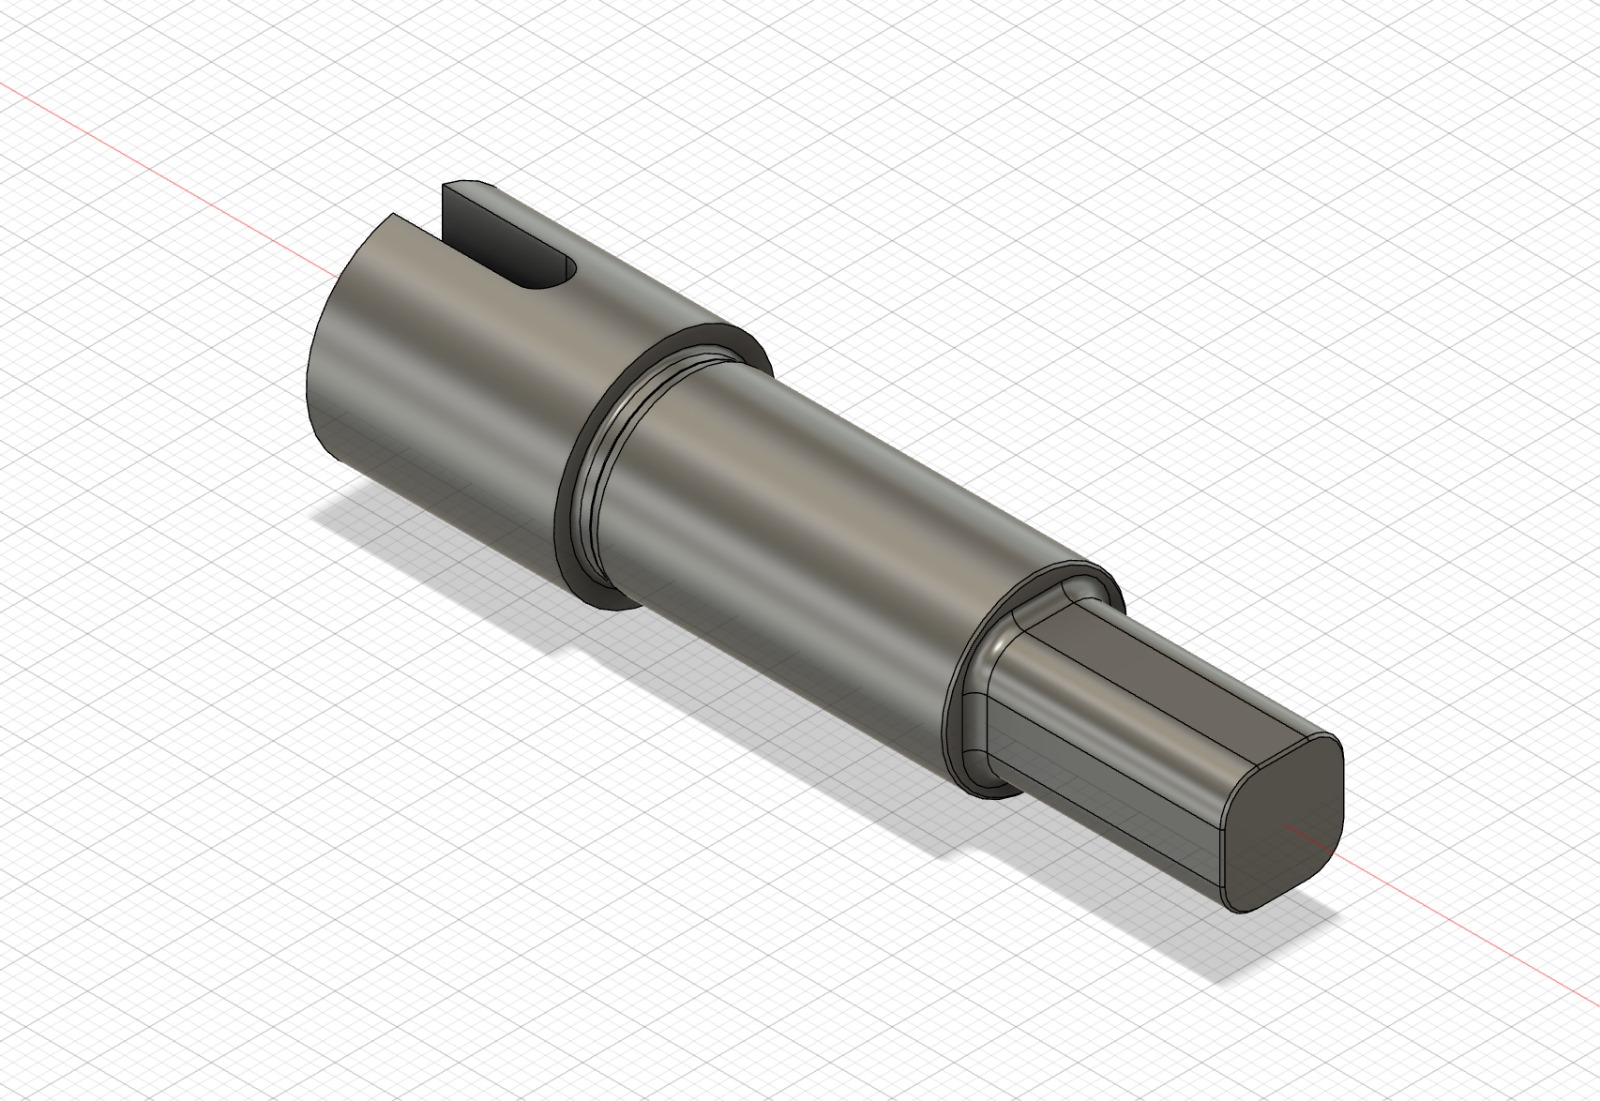
\includegraphics[width=0.5\textwidth]{hub_shaft.jpeg}
        \caption{Motor-Wheel Hub shaft, machined out of 6061-T6 aluminum}
        \label{fig:wheel-shaft-hub}
    \end{figure}


\section{Elasticity}

    The Young's Modulus and Elasticity between PLA and 6061-T6 aluminum showed differences when
    compared to one another, which suggests their different uses and stress resistance.

    Based on BCN3D Technologies' PLA datasheet \cite{pla_spec_ultimaker}, the material has Young's modulus of 3120 MPa (or
    roughly 3.2 GPa). The fact that PLA is a semi-crystalline polymer that was intended to be flexible and
    simple to produce can be seen in its low modulus score (link). The elasticity of PLA was moderate,
    meaning that it could deform under stress and return to its former shape when the load was released.

    % start figure environment
    \begin{figure}[H]
        \centering
        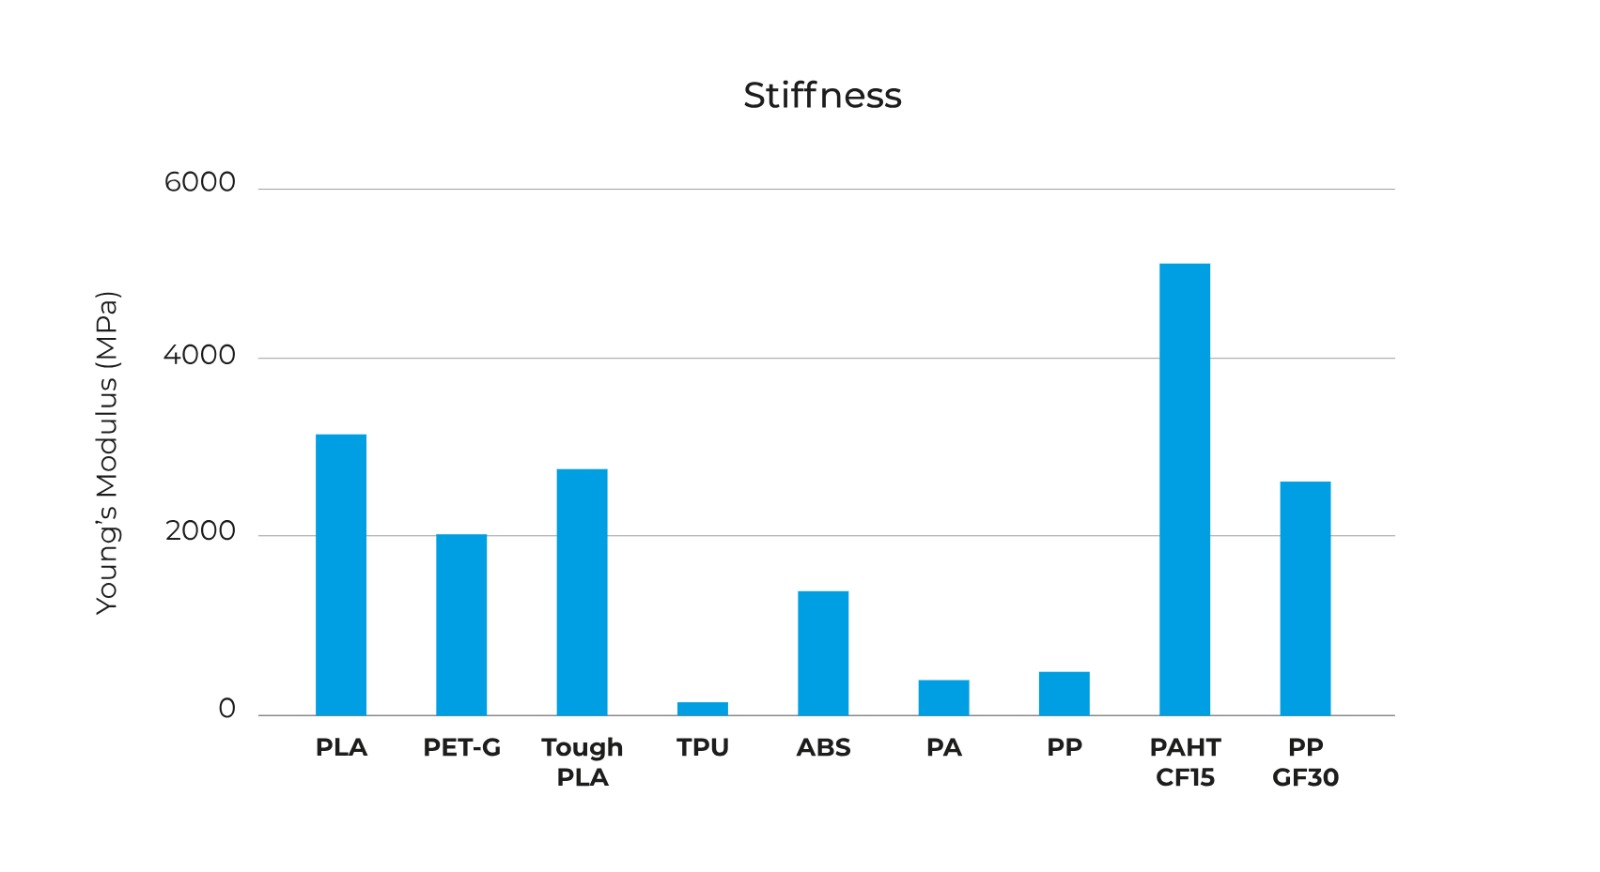
\includegraphics[width=0.5\textwidth]{PLA_stiffnes.jpeg}
        \caption{PLA Stiffness} 
        \label{fig:pla-stiffness}
        \cite{figure_materials_tensile}
    \end{figure}

    However, with certain components, the 3D-printed PLA could make it brittle. Therefore, it was appropriate
    for low-stress applications and prototyping where high rigidity was not a requirement. Elasticity in a
    material helped so that it could absorb some impact without permanent deformation, making it useful for
    lightweight and less structurally demanding parts.
    6061-T6 aluminum had a much greater Young's modulus of 68.9 GPa \cite{aluminum_spec}. Compared to PLA, 6061-T6
    aluminum was stiffer and had a smaller chance to deform under stress, as shown by its higher modulus.

    % start figure environment
    \begin{figure}[H]
        \centering
        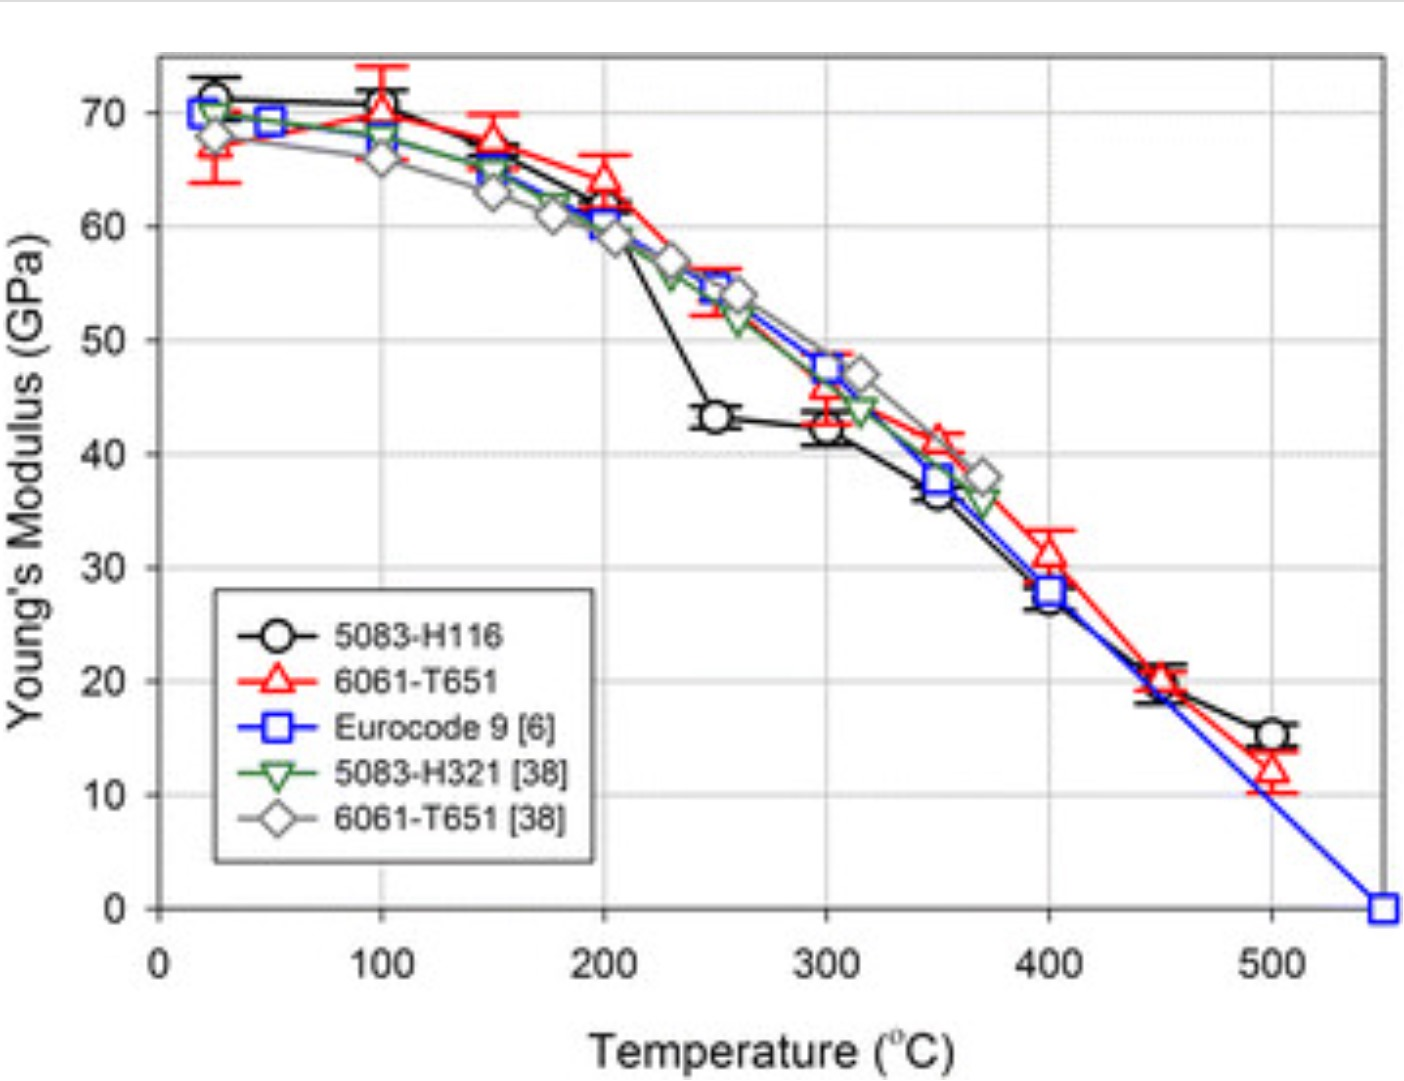
\includegraphics[width=0.5\textwidth]{alu_stiffness.jpeg}
        \caption{Aluminum Stiffness} 
        \label{fig:aluminum-stiffness} 
        \cite{Elasticity_graph_aluminium}

    \end{figure}

    The material was applicable in instances where rigidity and endurance were required due to its
    decreased elasticity, which allowed it to bear larger loads without experiencing significant deformation.
    The contrast in elasticity and Young's modulus between PLA and 6061-T6 aluminum showed the different uses for which each material was appropriate.
\section{Surface Quality}

    For 3D printed PLA, the noticeable layer lines on the surface were a result of the layer-by-layer
    deposition used in FDM (Fused Deposition Modelling) technology \cite{fusion_deposition_modeling}. The print resolution determined
    how smooth the surface was; surfaces with thinner layers at higher resolutions were smoother while at
    lower resolutions, layer lines were more apparent. To smooth and minimize roughness, post-processing
    methods like coating and sanding were used. Despite these initiatives, 3D-printed PLA had rougher
    surfaces than machined metals.

        % Add to figure environment
    \begin{figure}[H]
        \centering
        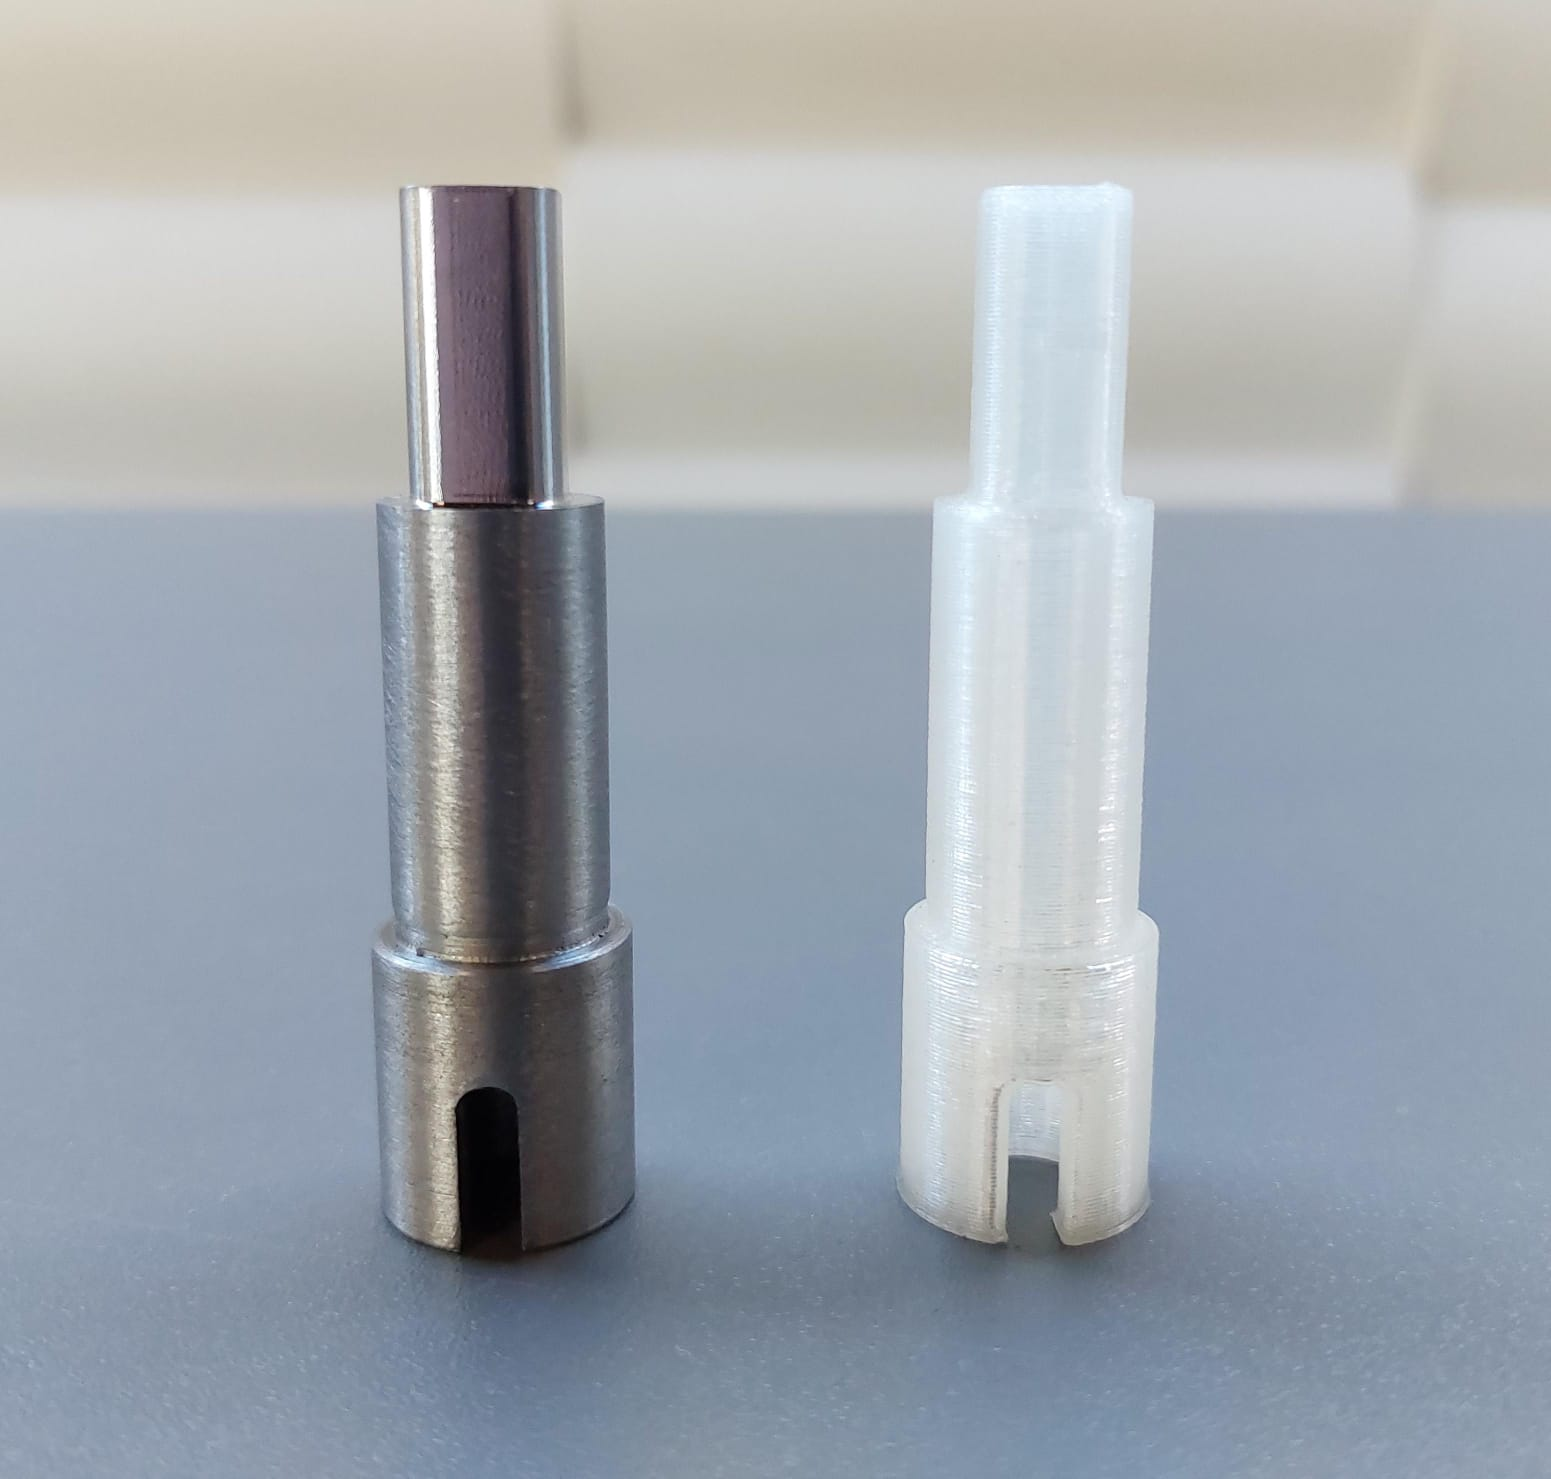
\includegraphics[width=0.5\textwidth]{alu_pla_surface.jpeg}
        \caption{3D Printed PLA Surface vs 6061-T6 Aluminum Surface}
        \label{fig:pla-surface}
    \end{figure}

    Next, components were made of 6061-T6 aluminum, which had a smoother surface and very little roughness
    (commonly at Ra 0.4 μm)\cite{aluminum_spec}. The components were produced with a certain degree of surface consistency
    and homogeneity due to the machining process. Moreover, surface quality could be improved by applying
    anodizing and polishing treatments, which would add a layer of protection and improve the appearance.
    6061-T6 Aluminium has a glossy natural finish and could possibly be polished even more to get a mirror-
    like surface, which makes it appealing and ideal for higher-end applications.

    In terms of aesthetics, 3D printed PLA parts could have had a matte to semi-glossy appearance, and
    depending on the filament used, there were a wide range of color options available, from typical white
    or transparent to several different colors available on the market.

    However, the components that were made from 6061-T6 aluminum had a silver-grey, natural glossy
    finish. This could have also had the possibility to be anodized in several colors, increasing the
    component's adaptability (get a link from MS chapters). If necessary, aluminum can be polished to a
    shinier finish which could increase the visual attractiveness and enable it for uses where performance
    and aesthetics are equally important.

\section{Thermal Properties}

    When choosing a material for a specific application, especially one where temperature changes are
    active, its thermal characteristics are important. Several differences between the thermal
    characteristics of 6061-T6 aluminum and 3D-printed PLA are apparent. Compared to metals, PLA has a
    lower melting point of 145 °C to 160 °C, which makes it acceptable for low-temperature applications. PLA
    components are also more prone to dimensional changes with temperature variations, which could
    impact their stability and precision in some applications. The coefficient of thermal expansion \cite{pla_spec_ultimaker} for PLA
    ranges from 68 to \(100\) x \(10^2\) °C. In addition, it loses its mechanical qualities and structural integrity due
    to thermal breakdown, which starts at temperatures higher than 200 °C.

    6061-T6 aluminum, on the contrary, has a much higher melting point between \(582\) °C and \(652\) °C making it ideal for high-temperature applications. Approximately \(23.6\) x \(10^2\)°C is the coefficient of
    thermal expansion of 6061-T6 aluminum, which is significantly lower than that of PLA and indicates a higher dimensional stability during temperature fluctuations. Furthermore, 6061-T6 aluminum retains its
    mechanical qualities and structural integrity across many circumstances and does not break down at
    normal operational temperatures. This comparison between the two materials emphasizes how important it is to choose the correct thermal requirements for an application. \cite{aluminum_spec}

\section{Precision}

    An analysis of the precision of parts manufactured from PLA using a Prusa MK4 3D printer and from
    6061-T6 aluminum using CNC machining or milling demonstrated differences in the two materials and
    processes in terms of dimensional accuracy, repeatability, complexity, and customization potential.

    With the Prusa MK4 dimensional accuracy for 3D printed parts usually varied between ±0.1 and ±0.2 mm \cite{prusa_mk4_precision},
    depending on variables which included: layer height, print speed, nozzle diameter, and printer calibration.
    The overall precision of the items was impacted by the inherent unpredictability introduced by the layer-by-layer deposition process of 3D printing. On the other hand, components made from 6061-T6 aluminum
    that were CNC machined or milled showed much better dimensional precision, with tolerances usually
    ranging from ±0.01 mm to ±0.003 mm \cite{cnc_milling_precision}. The machining procedure, equipment calibration, tool wear, and
    thermal expansion could have been variables that affected this precision.

    Another important factor was repeatability, or the ability to consistently make the same parts. When
    applying the same print parameters, the Prusa MK4 showed good repeatability, though small differences
    could happen due to environmental factors and the grade of the filament. Even though they are small,
    these differences could affect the way parts made in large quantities turn out. In contrast, high precision
    was provided by CNC machining 6061-T6 aluminum, guaranteeing almost identical parts within
    predetermined tolerances. This constancy would be essential for applications that needed accuracy and
    consistency between different units.

    Additionally, there were also notable differences in each manufacturing method's complexity and
    customization. Complex interior structures and geometries that were difficult or impossible to machine
    might be produced using the Prusa MK4. This feature, along with the simplicity and affordability of modifying
    and improving designs, enabled 3D printing a compelling choice for specific components and prototypes.

    Nevertheless, CNC machining could have had limitations and frequently be needed for specialized
    equipment, despite its ability to handle complicated geometries. In conventional manufacturing,
    customization would be more costly and time-consuming as it required much more labor and funds to
    change designs after the tooling was put up.
    \newpage

\section{Cost}

    Made from 3D Printing PLA:
    \begin{itemize}
        \item 4x Motor-Wheel Shaft: €0.76
        \item 2x Rocker Axle: €1.92
        \item 2x Boogie Axle: €1.48
        \item Total: €4.16
    \end{itemize}

    Made from 6061-T6 Aluminium:

    \begin{itemize}
        \item 4x Motor-Wheel Shaft
        \item 2x Rocker Axle
        \item 2x Boogie Axle
        \item Total: €201.28    
    \end{itemize}

    When comparing the price of parts produced of 6061 T6 Aluminium and PLA printed by a Prusa MK4, there
    was a noticeable price difference. The same components - 4x motor-wheel shafts, 2x Rocker Axles, and 2x Boogie Axles - were made with both materials. The entire cost of employing PLA 3D printing to produce
    these components was €4.16. The motor-wheel shafts cost €0.76, the rocker axles €1.92, and the boogie
    axles €1.48 according to the breakdown. This is a visible difference to the same components made out of
    6061-T6 aluminium which came to a total cost of €201.28.

    Despite the higher expense associated with 6061-T6 aluminum, it came down to the quality of the components that were produced. Aluminium was stronger, more resilient, and more durable than PLA,
    which when it came to specific components, was generally weaker than what was needed and was more
    prone to deterioration over time. Long-term cost-effectiveness was ensured by superior performance
    and fewer replacement needs for aluminum components, which nearly made up for their higher original
    cost.

    \newpage

\section{Time Comsumption}

    3D-P PLA:
    \begin{itemize}
        \item On Prusa MK4
        \item 2x Rocker Axle
        \item 2x Boogie Axle
        \item 4x Motor-Wheel Shaft
        \item All components were also made in one print (which means they all fit on the board)
        \item Total time (in hrs): 11 hours and 30 minutes
    \end{itemize}

    6061 T6 Aluminium:
    \begin{itemize}
        \item Went to Muharraq Engineering located in Manama, Bahrain
        \item Made the order on 25.05.2024 at 11h30
        \item Received all components 29.05.2024 at 15h30
        \item Total time (in hrs): 100 hours
    \end{itemize}

    There was an evident difference in the time efficiency when the production durations of the components
    made from 6061-T6 aluminum and PLA were compared. Using a Prusa MK4, the parts - which included
    4x motor-wheel shafts, 2x rocker axles, and 2x boogie axles - were created in a total of eleven hours
    and 30 minutes. This quick processing time and useful efficiency of 3D printing technology were shown by
    the rapid output that was achieved in a single print run. When it came to manufacturing the same
    components out of 6061-T6 aluminum, it took much longer. The parts were manufactured by Muharraq
    Engineering is located in Manama, Bahrain and took a total time of around 100 hours for the components to
    be produced. The order placement was made on May 25, 2024, at 11:30, and the component delivery was
    made on May 29, 2024, at 15:30.

    According to this comparison, the 3D printing method using PLA produced the components 8.7 times
    faster than the conventional manufacturing method using aluminum. 3D printing is a very useful
    technique for projects that have a tight deadline because of its speedy manufacturing capabilities, which
    enable quicker prototyping and shorter lead times. It should be mentioned nonetheless that the
    manufacturing time for the 6061-T6 aluminum components may change depending on the engineering
    firm and the particulars of the order. The aluminum components provide better strength and durability
    despite the longer production time, highlighting the balance between material quality and speed.

\section{Manufacturing Workflow Complexity}

    The process of producing a component using 3D printing PLA was considerably more
    straightforward compared to manufacturing the same component from 6061-T6 aluminum. The Prusa
    MK4 was simply loaded with an STL file to initiate the 3D printing process. Since no further technical
    procedures were needed to translate the digital content into a physical thing, this method required
    minimal preparation.

    In contrast, making a component out of 6061-T6 aluminum required a far more involved and repetitive
    procedure. The design had to be created in Fusion360, where detailed technical drawings were drawn up.
    For both accuracy and operation to be guaranteed, certain tolerances had to be finished and sent to an
    engineer for assessment. Several rounds of comments and revisions were frequently made during this
    review process. The developer would put the improvements into place after the engineer reviewed the
    drawing and made any necessary suggestions; occasionally, this might need multiple iterations before
    final permission was given.

    In the final stages, the component would be approved and then put in a manufacturing queue to wait to
    be made. Compared to the process of 3D printing with PLA, the procedure of design, review, correction,
    and approval, followed by scheduling for production, added a significant amount of time and complexity.

\section{Environmental Impact}

    Since the introduction of 3D printing and the use of PLA, it has gained a number of environmentally
    beneficial characteristics along the way. PLA had a sustainable material source as it was made from
    renewable resources like sugarcane and corn starch In
    general, 3D printing PLA required less energy than conventional manufacturing techniques for small
    quantities. Moreover, there was very little waste produced by additive manufacturing techniques. PLA has
    low biodegradability in ordinary landfill sites, but it could be biodegraded under industrial composting
    conditions when its lifespan comes to an end\cite{pla_environmental_impact1}\cite{pla_environmental_impact2}.

    When it comes to the ecological impact of manufacturing with 6061-T6 aluminum was different. Bauxite ore
    was extracted to provide the raw material for aluminum, a process that is extremely energy-intensive
    during the mining and processing stages. As a result, the energy required to produce 6061-T6 aluminum
    was much higher because of the machinery and energy it required for both mining and refining.
    Additionally, substantial amounts of waste were produced by subtractive manufacturing techniques often
    used to produce aluminum, including shavings and off-cuts. But 6061-T6 aluminum was highly
    recyclable at the end of its lifespan without losing any of its qualities. Aluminum recycling uses just
    around 5\% of the energy needed to make new aluminum from ore, making it a very energy-efficient
    process\cite{aluminium_environmental_impact1}\cite{aluminium_environmental_impact2}.

    Under certain circumstances, PLA was recyclable and biodegradable, but its actual recyclability was
    constrained by the capabilities of infrastructure. However, the recycling process for 6061-T6 aluminum
    was well-established and resulted in notable energy savings while preserving the material's
    characteristics. This comparison reinforced the necessity for sustainable practices in material selection
    and production processes by highlighting the importance of also choosing materials based on the
    environment and the potential to be recycled.